$$f : \mathbb{R} \longrightarrow \mathbb{R}^+,\ x \longmapsto b^x \ | b \in \mathbb{R}^+ \setminus \lbrace 1 \rbrace$$
\begin{tabular}[t]{cc}
    $f : \mathbb{R} \longrightarrow \mathbb{R}^+,\ x \longmapsto 2^x$ & $f*^{-1} : \mathbb{R}^+ \longrightarrow \mathbb{R},\ x \longmapsto \log_2(x)$ \\
    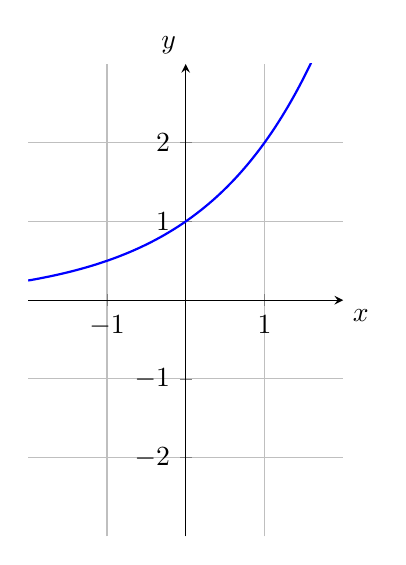
\begin{tikzpicture}
        \begin{axis}
            [
            x = 1cm, y = 1cm,
            xmin = -2, xmax = 2,
            ymin = -3, ymax = 3,
            axis lines = center,
            xtick={-1,0,...,1},
            ytick={-2,-1,...,2},
            xlabel={$x$},
            ylabel={$y$},
            xlabel style={below right},
            ylabel style={above left},
            grid=both]
            \addplot[
                domain = -2:2,
                samples = 200,
                smooth,
                thick,
                blue,
            ] {2^x};
        \end{axis}
    \end{tikzpicture}                                                 &
    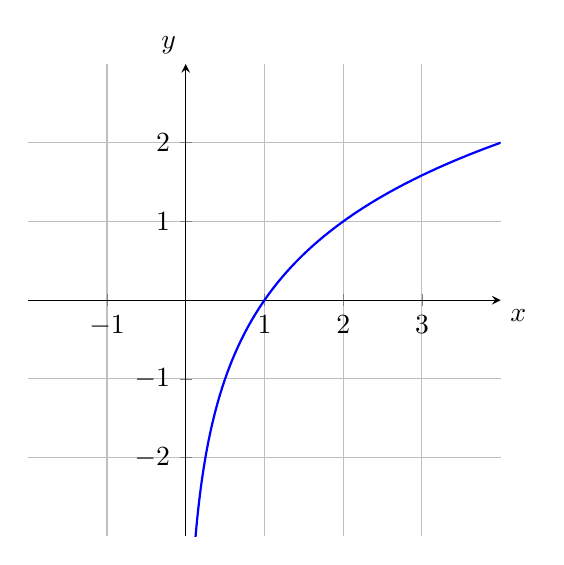
\begin{tikzpicture}
        \begin{axis}
            [
            x = 1cm, y = 1cm,
            xmin = -2, xmax = 4,
            ymin = -3, ymax = 3,
            axis lines = center,
            xtick={-1,0,...,3},
            ytick={-2,-1,...,2},
            xlabel={$x$},
            ylabel={$y$},
            xlabel style={below right},
            ylabel style={above left},
            grid=both]
            \addplot[
                domain = -0.01:4,
                samples = 200,
                smooth,
                thick,
                blue,
            ] {ln(x)/ln(2)};
        \end{axis}
    \end{tikzpicture}
\end{tabular}
